\documentclass[10pt]{article}

\def\Type{LessonCaelan}
\def\TypeNum{Lesson 3}
\def\TypeTitle{Limits and Continuity \\Notes to Instructors}
\def\Semester{Fall 2021} %Not Used 
\def\Course{MATH 1190 \& 1210}
\def\Targets{ {\bf\color{RoyalBlue}L1}, {\bf\color{RoyalBlue}L1} }

\usepackage{preambleDJ}





%%%%%%%%%%%% BEGIN DOCUMENT %%%%%%%%%%%%%%%
%%%%%%%%%%%% BEGIN DOCUMENT %%%%%%%%%%%%%%%
%%%%%%%%%%%% BEGIN DOCUMENT %%%%%%%%%%%%%%%
%%%%%%%%%%%% BEGIN DOCUMENT %%%%%%%%%%%%%%%
%%%%%%%%%%%% BEGIN DOCUMENT %%%%%%%%%%%%%%%

\begin{document}


\thispagestyle{firstpage}
\pagestyle{otherpages}
\vs{.5}
\lt  
\enumC{
\item[\target{L1}:] Limits and Continuity
\itemC{
    \item State and give graphical/formulaic examples of the three continuity conditions. 
    \item Identify and classify types of discontinuity based on the definition of continuity.  
}
}

\enumC{
\item[\target{L2}:] Evaluate Limits Using Continuity and Forms
\itemC{
    \item Evaluate limits using continuity. 
}
}

~\\

\lg Students will be able to...
\enumCN{
\item Describe informally and formally what it means for a function to be continuous.
\item Identify $3$ continuity conditions.
\item Connect $3$ continuity conditions with different kinds of discontinuities (removable, jump, infinite). 
\item Use Main Continuity Theorem to evaluate limits.  
\item Use $3$ Practical Rules to determine domain of a continuous function.
\item Sketch functions that meet given continuity conditions.
}

\feed
\itemC{
\item Some thought the videos were long but understandable.
\item Some thought videos were disengaging.
\item Others did not understand continuity conditions.
\item Others need more practice identifying different kids of discontinuities (jump, removable, infinite).
}
 \hand
 \itemI{
 \item Mini-lecture page 1 is intended to connect finding limits from last class period (examining trends towards $x=a$ but ignoring $f(a)$) with special case when $\ds \limx[a]f(x)=f(a)$. This leads to informal/formal descriptions of continuity. Example/Exercise reinforce fact that continuity allows us to evaluate limits. We come back to this idea later when we talk about Main Continuity Theorem.
 \item Page $2$ highlights $3$ continuity conditions and how they connect with definition of continuity.  Practice ensues!
 \item Main Continuity Theorem allows us to build complicated (continuous) functions from basic (continuous) building blocks.  We need practical guidance to determine when a value is in the domain, so we have $3$ Practical Rules.
 \item Example 2/Exercise B and Example 3 and Exercise D give practice identifying whether or not a value is in domain of given function.
 \item {\bf Extra Practice 1} is great prep for exam. If students can handle this question, they understand a lot.
 }

\core Exercise B, Example 2/Exercise C, Example 3, Exercise D.


\newpage


\textbf{Intended Learning Outcomes}
After this lesson, you will be able to 

\begin{itemize}
    \item State and give graphical/formulaic examples of the three continuity conditions. (\target{L1})
    \item Identify and classify types of discontinuity based on the definition of continuity. (\target{L1})
    \item Evaluate limits using continuity. (\target{L2})
\end{itemize}

\vspace{-0.5cm}

\hrulefill

\vspace{0.3cm}

\minil \mod Last time together, we explored the idea and notation of limits.\\
%\vs{-.2}
   \mpageTth{.25}{.4}{.35}{
  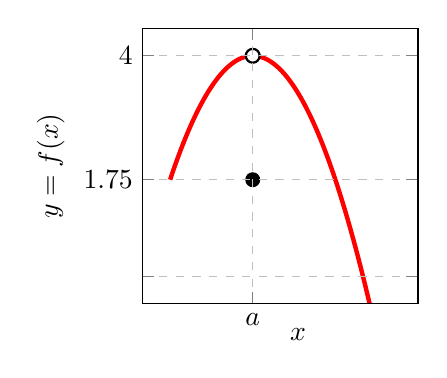
\begin{tikzpicture}[scale=1]
          \begin{axis}[
        %    axis y line = left,
        %    axis x line = bottom,
            xlabel={$x$},
            xtick       = {1.5},
            xticklabels = {$a$},
            ytick       = {0,1.75,4},
            yticklabels = {,$1.75$,$4$},
            samples     = 160,
            domain      = -1:5,
            restrict y to domain=-1:5,
            xmin = -0.5, xmax = 4.5,
            ymin = -0.5, ymax = 4.5,
            grid=both, grid style=dashed,
            width=2in, height=2in,
            y label style={anchor=south},
            ylabel={$y=f(x)$},
        		axis on top,
		x label style={anchor=west},
          ]
          % pieces 1 and 2
          \addplot[domain=0:5, red, ultra thick, mark=none] {4-(x-1.5)^2};
          \filldraw[white] (1.5,4) circle (2.5pt);
          \draw[thick] (1.5,4) circle (2.5pt);
             \filldraw[black] (1.5,1.75) circle (2.5pt);
        \end{axis}
        \end{tikzpicture}
  }{
  \vs{.2}
          \itemI{
		\item As $x$ gets close to $a$ (from the left) the trend of $f(x)$ is towards $4$. \vs{.1}
		\item As $x$ gets close to $a$ (from the right) the trend of $f(x)$ is towards $4$. \vs{.1}
		\item As $x$ gets close to $a$ the trend of $f(x)$ is towards $4$. \vs{.1}
		\item $f(a)=1.75$\vs{.3}
        }
   }{
  \centering {\bf Notation/Observations}
    \nti{
  \itemI{
  \item$\ds \lim_{x\to 4^-}f(x)=4$
  \item$\ds \lim_{x\to 4^+}f(x)=4$  \vs{.1}
    \item$\ds \lim_{x\to 4}f(x)=4$  
    \item Whether limit exists (or not) does not depend on $f(a)$, i.e. the $y$-value exactly at $x=a$.
  }
  }
  }
  \vs{-.2}
  \hrule
  ~\\
%  \vs{-.3}
   \mpageTth{.25}{.4}{.35}{
   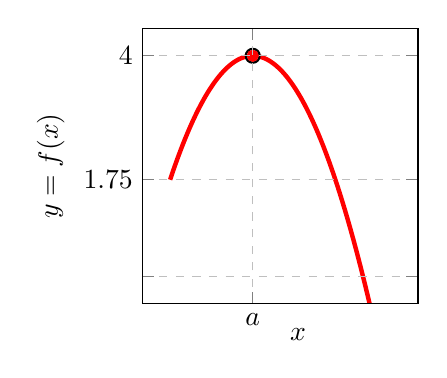
\begin{tikzpicture}[scale=1]
          \begin{axis}[
        %    axis y line = left,
        %    axis x line = bottom,
            xlabel={$x$},
            xtick       = {1.5},
            xticklabels = {$a$},
            ytick       = {0,1.75,4},
            yticklabels = {,$1.75$,$4$},
            samples     = 160,
            domain      = -1:5,
            restrict y to domain=-1:5,
            xmin = -0.5, xmax = 4.5,
            ymin = -0.5, ymax = 4.5,
            grid=both, grid style=dashed,
            width=2in, height=2in,
            y label style={anchor=south},
            ylabel={$y=f(x)$},
        		axis on top,
		x label style={anchor=west},
          ]
          % pieces 1 and 2
          \addplot[domain=0:5, red, ultra thick, mark=none] {4-(x-1.5)^2};
          \filldraw[white] (1.5,4) circle (2.5pt);
          \draw[thick] (1.5,4) circle (2.5pt);
             \filldraw[red] (1.5,4) circle (2.pt);
        \end{axis}
        \end{tikzpicture}
  }{
\vs{.2} \itemI{
		\item As $x$ gets close to $a$ (from the left) the trend of $f(x)$ is towards $4$. \vs{.1}
		\item As $x$ gets close to $a$ (from the right) the trend of $f(x)$ is towards $4$. \vs{.1}
		\item As $x$ gets close to $a$ the trend of $f(x)$ is towards $4$. \vs{.1}
		\item $f(a)=\blue{4}$ \vs{.3}
        }
  }{
  \centering {\bf Notation/Observations}
      \nti{
  \itemI{
  \item$\ds \lim_{x\to 4^-}f(x)=4$
  \item$\ds \lim_{x\to 4^+}f(x)=4$  \vs{.1}
    \item$\ds \lim_{x\to 4}f(x)=4$  
    \item In this example, $f(a)$ is initially undefined.  However, if we "fill in the hole" and let $f(a)=4$, we have a special situation where the limit also equals the the $y$-value at $x=a$. We say {\em $f(x)$ is continuous at $x=a$.}
  }
  }
  }
\vs{-.2}
  \hrule ~\\
\mpageT{.5}{.5}[\hs{.2}]{
\begin{center}{\bf \blue{Informal Key Idea:}} \end{center}
A function is {\em continuous} when you don't have to lift your writing utensil when sketching the graph.
\vs{.25}~\\
{\bf\blue{Why do we care about continuity?}}
\itemC{
\item Cooling of an object \vs{.05}
\item Behavior of electronic circles \vs{.05}
\item Fluid flow over an airplane wing\vs{.05}
\item Many others...\vs{.05}
\item \blue{\bf Computing Limits! }
}
}{
\begin{center}\blue{\bf Formal Key Idea:}\\
A function is {\em continuous} at a number $a$  when \\
\centering \blue{$\ds \lim_{x \to a}f(x)=f(a)$}\end{center}
\nti{One of the important implications of this is that we can use this to find limits involving continuous functions. Up until this point, we've had to examine tables of data or use the graph of a function to infer limits.  Thus continuity is something that might be helpful to us when when we don't have tables of data or graphs available to us.  Examples follow...}
}

\mpageT{.5}{.5}[\hs{.15}]{
\example \ltrm{\color{RoyalBlue}L2} $\ds f(x)=\frac{x^2+1}{x-2}$ is continuous at $x=3$. Find $\ds \lim_{x\to3} \frac{x^2+1}{x-2}$ 
\sol{
We are told that $\ds f(x)=\frac{x^2+1}{x-2}$ is continuous at $x=3$. Thus, $$ \limx[3] f(x)=f(3)=\frac{3^2+1}{3-2}=\frac{10}{1}=10$$
}
}{
{\exercise }  $\ds f(x)=\frac{\sqrt{x+5}}{x+2}$ is continuous at $x=4$. Find $\ds \lim_{x\to4} \frac{\sqrt{x+5}}{x+2}$.
\sol{
We are told that $\ds f(x)=\frac{x^2+1}{x-2}$ is continuous at $x=4$. Thus, $$ \limx[4] f(x)=f(4)=\frac{\sqrt{4+5}}{4+2}=\frac{3}{6}=\frac{1}{2}$$
}
}
%%%%%%%%%%%%%

\mod In the pre-class assignment, you saw the definition of continuity, as well as different types of discontinuities. The goal of this lesson is to learn how to use the definition of continuity to decide whether a function is continuous at a number and to discern between different types of discontinuities.\\

{\bf \textcolor{blue}{Fill in the blanks!}} The pre-class assignment for today's lesson covered the formal {\bf definition of continuity}. 
\begin{center}
{\it The function $f$ is continuous at the number $a$ provided $\displaystyle\lim_{x\to a} f(x)=f(a)$.} \\ % for NTI \unline{.75}{$f(a)$}{.15}
\end{center}

\bigskip

This short definition can be broken up into {\bf three continuity conditions} -- can you remember what they are? The function $f$ is continuous at $a$ provided...  \\
\nti{I'm going to point to definition above and comment about how following 3 conditions flow out of definition.}
(1) $f(a)$ \unline{1}{\blue{is defined}}{.15}  \hfill
%
(2) $\displaystyle\lim_{x\to a}f(x)$ \unline{1}{\blue{exists}}{.15}\hfill
%
(3) \unline{2}{\blue{(1)=(2),i.e.  $\ds \limx[a]f(x)=f(a)$}}{.15} \\[0.3in]

{\bf \blue{Key Question: When is a function {\em not} continuous?}}\\
{\exercise{\color{RoyalBlue} L1}} Given below are graphs of functions discontinuous at $a$:\\

\,\hfill
        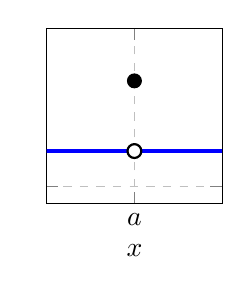
\begin{tikzpicture}[scale=1]
          \begin{axis}[
        %    axis y line = left,
        %    axis x line = bottom,
            xlabel={$x$},
            xtick       = {2},
            xticklabels = {$a$},
            ytick       = {0},
            yticklabels = {},
            samples     = 160,
            domain      = -1:5,
            restrict y to domain=-1:5,
            xmin = -0.5, xmax = 4.5,
            ymin = -0.5, ymax = 4.5,
            grid=both, grid style=dashed,
            width=1.5in, height=1.5in
          ]
          % pieces 1 and 2
          \addplot[domain=-1:5, blue, ultra thick, mark=none] {1};
          \filldraw[white] (2,1) circle (2.5pt);
          \draw[thick] (2,1) circle (2.5pt);
          \filldraw[black] (2,3) circle (2.5pt);
        \end{axis}
        \end{tikzpicture}
        %
        \hfill
        %
        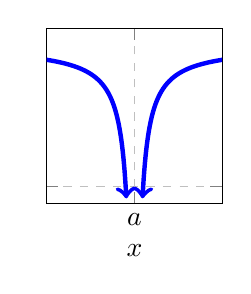
\begin{tikzpicture}[scale=1]
          \begin{axis}[
        %    axis y line = left,
        %    axis x line = bottom,
            xlabel={$x$},
            xtick       = {2},
            xticklabels = {$a$},
            ytick       = {0},
            yticklabels = {},
            samples     = 160,
            domain      = -1:5,
            restrict y to domain=-1:5,
            xmin = -0.5, xmax = 4.5,
            ymin = -0.5, ymax = 4.5,
            grid=both, grid style=dashed,
            width=1.5in, height=1.5in
          ]
          % pieces 1 and 2
          \addplot[domain=-1:1.77, blue, ultra thick, mark=none, <->] {4-abs(x-2)/(x-2)^2};
           \addplot[domain=2.23:5, blue, ultra thick, mark=none, <->] {4-abs(x-2)/(x-2)^2};
        \end{axis}
        \end{tikzpicture}
        %
        \hfill
        %
        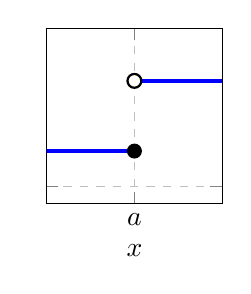
\begin{tikzpicture}[scale=1]
          \begin{axis}[
        %    axis y line = left,
        %    axis x line = bottom,
            xlabel={$x$},
            xtick       = {2},
            xticklabels = {$a$},
            ytick       = {0},
            yticklabels = {},
            samples     = 160,
            domain      = -1:5,
            restrict y to domain=-1:5,
            xmin = -0.5, xmax = 4.5,
            ymin = -0.5, ymax = 4.5,
            grid=both, grid style=dashed,
            width=1.5in, height=1.5in
          ]
          % pieces 1 and 2
          \addplot[domain=-1:2, blue, ultra thick, mark=none] {1};
          \filldraw[black] (2,1) circle (2.5pt);
          \addplot[domain=2:5, blue, ultra thick, mark=none] {3};
          \filldraw[white] (2,3) circle (2.5pt);
          \draw[thick] (2,3) circle (2.5pt);
        \end{axis}
        \end{tikzpicture}
        %
        \hfill
        %
        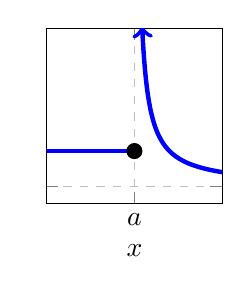
\begin{tikzpicture}[scale=1]
          \begin{axis}[
        %    axis y line = left,
        %    axis x line = bottom,
            xlabel={$x$},
            xtick       = {2},
            xticklabels = {$a$},
            ytick       = {0},
            yticklabels = {},
            samples     = 160,
            domain      = -1:5,
            restrict y to domain=-1:5,
            xmin = -0.5, xmax = 4.5,
            ymin = -0.5, ymax = 4.5,
            grid=both, grid style=dashed,
            width=1.5in, height=1.5in
          ]
          % pieces 1 and 2
          \addplot[domain=-1:2, blue, ultra thick, mark=none] {1};
          \filldraw[black] (2,1) circle (2.5pt);
          \draw[thick] (2,1) circle (2.5pt);
          \addplot[domain=2.22:5, blue, ultra thick, mark=none, <->] {1/(x-2)};
        \end{axis}
        \end{tikzpicture}
        %
        \hfill
        %
        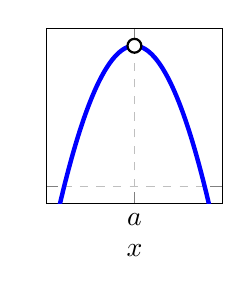
\begin{tikzpicture}[scale=1]
          \begin{axis}[
        %    axis y line = left,
        %    axis x line = bottom,
            xlabel={$x$},
            xtick       = {2},
            xticklabels = {$a$},
            ytick       = {0},
            yticklabels = {},
            samples     = 160,
            domain      = -1:5,
            restrict y to domain=-1:5,
            xmin = -0.5, xmax = 4.5,
            ymin = -0.5, ymax = 4.5,
            grid=both, grid style=dashed,
            width=1.5in, height=1.5in
          ]
          % pieces 1 and 2
          \addplot[domain=-1:5, blue, ultra thick, mark=none] {4-(x-2)^2};
          \filldraw[white] (2,4) circle (2.5pt);
          \draw[thick] (2,4) circle (2.5pt);
        \end{axis}
        \end{tikzpicture}
        %
        \hfill
        %
        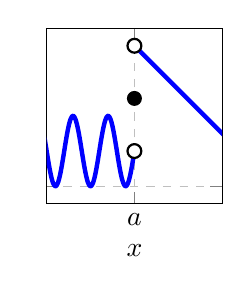
\begin{tikzpicture}[scale=1]
          \begin{axis}[
        %    axis y line = left,
        %    axis x line = bottom,
            xlabel={$x$},
            xtick       = {2},
            xticklabels = {$a$},
            ytick       = {0},
            yticklabels = {},
            samples     = 160,
            domain      = -1:5,
            restrict y to domain=-1:5,
            xmin = -0.5, xmax = 4.5,
            ymin = -0.5, ymax = 4.5,
            grid=both, grid style=dashed,
            width=1.5in, height=1.5in
          ]
          % pieces 1 and 2
          \addplot[domain=-1:2, blue, ultra thick, mark=none] {1+sin(deg(x)*3.141*2)};
          \filldraw[white] (2,1) circle (2.5pt);
          \draw[thick] (2,1) circle (2.5pt);
          \addplot[domain=2:5, blue, ultra thick, mark=none] {6-x};
          \filldraw[white] (2,4) circle (2.5pt);
          \draw[thick] (2,4) circle (2.5pt);
          \filldraw (2,2.5) circle (2.5pt);
        \end{axis}
        \end{tikzpicture}
    \hfill\,\\

\,\hfill 
\unline{.8}{\blue{RD, $3$}}{.1}
\hfill 
\unline{.8}{\blue{ID, $1,2,3$}}{.1}
\hfill 
\unline{.8}{\blue{JD, $2,3$}}{.1}
\hfill 
\unline{.8}{\blue{ID, $2,3$}}{.1}
\hfill 
\unline{.8}{\blue{RD, $1,3$}}{.1}
\hfill 
\unline{.8}{\blue{JD, $2,3$}}{.1}
\hfill\,\\
%
\enumC{
\item[i.] For each graph above, label the graph as depicting a removable, jump, or infinite discontinuity by writing the letters ``RD", ``JD", or ``ID" (respectively) in the blank below the graph.\\
\item[ii.] If a function is discontinuous at a number, then the function must violate at least one of the three conditions you wrote in the fill-in-the-blanks exercise. For each graph above, label the graph with the number(s) of the continuity condition(s) the graph violates in the space below the graph.\\
\item[iii.] Based on your labeling, characterize each type of discontinuity by which continuity conditions must be violated.

\itemC{
\item $f$ has a {\bf removable} discontinuity at $a$ {\it always} means continuity condition(s) \unline{.75}{\blue{$3$}}{.125} are violated.\\\\
\item $f$ has a {\bf jump} discontinuity at $a$ {\it always} means continuity condition(s)\unline{.75}{\blue{$2, 3$}}{.125} is/are violated.\\\\
\item $f$ has an {\bf infinite} discontinuity at $a$ {\it always} means continuity condition(s) \unline{.75}{\blue{$2, 3$}}{.125} is/are violated.  \blue{The fact that we have an {\em infinite} discontinuity means that at least one of the one-sided limits is $\pm \infty$}
}

}

%%%%%%%%%
%
%%%%%%%%%

{\bf\color{blue}When can we be confident that a function {\em is} continuous?} The pre-class assignment for today's lesson covered the Main Continuity Theorem and the Rules for Finding Domains:
%
\important{The Main Continuity Theorem}
{
%
\,\\[-0.05in]
%
Any function that is some combination \blue{($+$, $-$, $\times$, $\div$, powers or compositions)}\\  of other continuous functions\\
 (polynomials, \hfill roots, \hfill   trigonometric functions, \hfill exponentials, logarithms, \hfil or absolute value)
\\
 \blue{\small $x^7-1$, $6x+2x^2$, etc.} \hs{.05}\blue{\small $\sqrt{x}$, $\sqrt[3]{x}$, etc.}\hs{.05}\blue{\small $\sin(x)$, $\cos(x)$, etc.}\hs{.5}\blue{\small $2^x$, $e^x$, $\ln(x)$, $\log_{10}(x)$, $|x|$, etc.}
\vs{.1}\\
is continuous on its \unline{1}{\blue{domain}}{.15}.
%
}

 {\bf \blue{Practical Rules for determining when a number is {\em not} in a domain}}\\
 A number is {\em not} in the domain when one of the following situations occur
 % problems Therefore, determining where familiar functions are continuous involves finding the domain of those functions, so let's record the rules for finding domains.
~\\
\mpageT{.8}{.3}{
\begin{itemize}
\item{\bf Rule \#1:} \blue{{\bf Division by $0$.}  If $\ds y=\frac{1}{x-2}$ this will occur when $x=2$.\\ See  example on the right.}  \\%Division by $0$ 
\end{itemize}
}{
 \begin{tikzpicture}[scale=.7]
          \begin{axis}[
        %    axis y line = left,
        %    axis x line = bottom,
            axis line style={line width=1.5pt}, % Adjust line width as needed for boldness
    % other axis options
            xlabel={$x$},
            x label style={anchor=west},
            xtick       = {1,2,3,4},
            xticklabels = {},
            ytick       = {-4,-3,-2,-1,1,2,3,4},
            yticklabels = {},
            samples     = 160,
            domain      = -1:4.5,
            restrict y to domain=-4:4,
            xmin = -2, xmax = 6,
            ymin = -4, ymax = 4,
            grid=both, grid style=dashed,
            width=2in, height=2in
          ]
          % pieces 1 and 2
          \addplot[domain=2:6, blue, ultra thick, <->] {1/(x-2)};
           \addplot[domain=-2:2, blue, ultra thick, <->] {1/(x-2)};
          \node at (4.3,-1.5) {$y=\dfrac{1}{x-2}$};
          \draw[dashed, red, ultra thick]  (2,-4) -- (2,4);
%          \addplot[domain=-0.5:4.5, ForestGreen, ultra thick, <->] {x^2};
%          \node at (1,4) {$e^x$};
%          \addplot[domain=-0.5:4.5, Goldenrod, ultra thick, ->] {x^(1/2)};
%          \node at (4,2.5) {$\sqrt{x}$};
%          \addplot[domain=0.6:4.5, red, ultra thick, <->] {ln(x)};
%          \node at (4,1) {$\ln(x)$};
        \end{axis}
    \end{tikzpicture}
  }
  ~\\
  \mpageT{.8}{.3}{
  \begin{itemize}
\item{\bf Rule \#2:} \blue{{\bf Even roots of negative numbers.} \\For example $y=\sqrt{x}$, $y=\sqrt[4]{x}$, $y=x^{1/6}$, etc..\\In graph on right, we see $y=\sqrt{x}$ is not defined for $x<0$ (but is at $x=0$).} \\ %Even roots of negative numbers
\end{itemize}
}{
 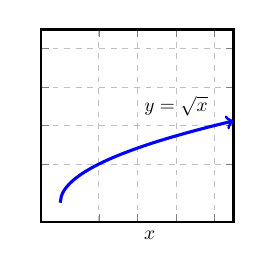
\begin{tikzpicture}[scale=.7]
          \begin{axis}[
        %    axis y line = left,
        %    axis x line = bottom,
            axis line style={line width=1.5pt}, % Adjust line width as needed for boldness
    % other axis options
            xlabel={$x$},
            x label style={anchor=west},
            xtick       = {1,2,3,4},
            xticklabels = {},
            ytick       = {1,2,3,4},
            yticklabels = {},
            samples     = 160,
            domain      = -1:4.5,
            restrict y to domain=-1:4.5,
            xmin = -0.5, xmax = 4.5,
            ymin = -0.5, ymax = 4.5,
            grid=both, grid style=dashed,
            width=2in, height=2in
          ]
%
          \addplot[domain=0:4.5, blue, ultra thick, ->] {x^(1/2)};
          \node at (3,2.5) {$y=\sqrt{x}$};
        \end{axis}
    \end{tikzpicture}
 }
 ~\\
   \mpageT{.8}{.3}{
  \begin{itemize}
\item{\bf Rule \#3:} \blue{{\bf Log of $0$ or negative number.}\\ For example $y=\ln(x)$, $y=\log_{10}(x)$, etc. We see on graph that $y=\ln(x)$ is not defined for $x\leq0$. In particular, there is a vertical axis at $x=0$.}\\ % Log of $0$ or negative number
\end{itemize}
}{
 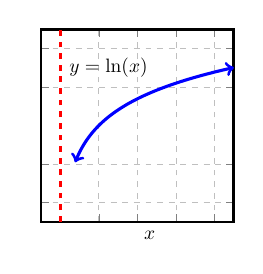
\begin{tikzpicture}[scale=.7]
          \begin{axis}[
        %    axis y line = left,
        %    axis x line = bottom,
	   axis line style={line width=1.5pt}, % Adjust line width as needed for boldness
    % other axis options
            xlabel={$x$},
            x label style={anchor=west},
            xtick       = {1,2,3,4},
            xticklabels = {},
            ytick       = {-4,-3,-2,-1,1,2,3,4},
            yticklabels = {},
            samples     = 160,
            domain      = -1:4.5,
            restrict y to domain=-1:4.5,
            xmin = -0.5, xmax = 4.5,
            ymin = -2.5, ymax = 2.5,
            grid=both, grid style=dashed,
            width=2in, height=2in
          ]
          \addplot[domain=0.05:4.5, blue, ultra thick, <->] {ln(x)};
          \node at (1.25,1.5) {$y=\ln(x)$};
                    \draw[dashed, red, ultra thick]  (0,-4) -- (0,4);
        \end{axis}
    \end{tikzpicture}
}~\\\\


\example{\color{RoyalBlue}L2}/ \exercise{\color{RoyalBlue}L2} For each of the following limits, decide whether the Main Continuity Theorem applies. If the theorem applies, then find the limit. If the theorem does not apply, then explain why.
\tasksA{2}{
\task ({\bf\color{blue}Example}) $\displaystyle\lim_{x\to-1}\dfrac{x+1}{x-1}$ 
\sol{
All components of function are continuous $x$, $1$, and $-1$. $x=-1$ is in domain, so $$\ds \limx[-1] f(x)=f(-1)=\frac{-1+1}{-1-1}{=0}{-2}=0$$
}
\task ({\bf\color{blue}Example}) $\displaystyle\lim_{x\to1}\dfrac{1}{\sqrt{x-1}}$ 
\sol{
When $x=1$, we have a division by $0$.
$$\frac{1}{\sqrt{1-1}}=\frac{1}{0}$$
Thus $x=1$ is {\em not} in the domain and theorem cannot be used.
}
task ({\bf\color{blue}Exercise}) $\displaystyle\lim_{x\to1}\dfrac{x+1}{x-1}$\sol{
We have division by $0$ when  $x=1$.
$$\frac{1+1}{1-1}=\frac{2}{0}$$
Thus $x=1$ is {\em not} in the domain and  Continuity Theorem does not apply.
}
\task ({\bf\color{blue}Exercise}) $\displaystyle\lim_{x\to3}\dfrac{x^3+1}{x-3}$
\sol{
When $x=3$ we have division by $0$. Thus $x=3$ is {\em not} in the domain and the Continuity Theorem does not apply.
}
\task ({\bf\color{blue}Exercise}) $\displaystyle\lim_{x\to0}\dfrac{1}{\sqrt{x-1}}$ 
\sol{
We have square root of a negative number when $x=0$
$$\frac{1}{\sqrt{0-1}}=\frac{1}{\sqrt{-1}}$$
Thus $x=0$ is {\em not} in the domain and theorem cannot be used.
}
\task ({\bf\color{blue}Exercise}) $\displaystyle\lim_{x\to4}\dfrac{\sqrt{x^2-4}+1}{x-7}$
\sol{
All components are continuous: $x^2-4$, $\sqrt{x^2-4}$, $1$, $x$, $7$.  $x=4$ is in the domain, so 
$$\limx[4] f(x)=f(4)=\frac{\sqrt{4^2-4}+1}{4-7}=\frac{\sqrt{12}+1}{-3}$$
}
}

\tasksAS{2}{6}{
\task ({\bf\color{blue}Extra Practice}) $\displaystyle\lim_{x\to0}\dfrac{x-2}{e^x-1}$
\sol{
We have division by $0$ when $x=0$.
$$ \frac{0-2}{e^0-1}=\frac{-2}{1-1}=\frac{-2}{0}$$
Thus $x=0$ is {\em not} in the domain and theorem cannot be used.  
}
\task ({\bf\color{blue}Extra Practice}) $\displaystyle\lim_{x\to2}\dfrac{x-2}{e^x-1}$
\sol{
All components are continuous: $x$, $2$, $e^x$, $1$. $x=2$ is in the domain. Thus
$$\limx[2] f(x) = f(2) = \frac{2-2}{e^2-1}=\frac{0}{e^2-1}=0$$
}
}

\vs{1}
\newpage

\example{\color{RoyalBlue}L1} Some very powerful mathematics we will learn later this semester depends upon being able to identify whether a function is continuous on an interval of $x$-values. Let's practice that skill here!\\

On which of the following intervals is $f(x)=\dfrac{\ln(x)}{x-4}$ continuous? Circle all that apply, and explain below.
\tasksA{4}{
\task  $[5,8]$ 
\task $[0,2]$ 
\task $[1,5]$ 
\task $[-7,-1]$ 
}

\nti{Feel free to convert this Example to an Exercise for students to work.}
\sol{
\itemI{
\item We note that when $x=4$, we have a division by $0$: $\ds \frac{\ln(4)}{4-4}=\frac{\ln(4)}{0}$. So $x=4$ is {\em not} in the domain. This is the only one of our $3$ Practical Rues for determining what is {\em not} in the domain that is relevant (see prior page).\\
\\
We eliminate any interval above that contains $1$. That leaves us with three intervals that do not contain $x=4$:\\
a) $[5,8]$, b) $[0,2]$  and d) $[-7,-1]$ 
\item $\ln(x)$ is not continuous for $x\leq 0$ so we eliminate any interval that contains $0$ or a negative value. This leaves the interval $[5,8]$ as the only option where $f(x)$ is continuous.
}
}
\vs{1}


\exercise{\color{RoyalBlue}L1} Give 1 example of an interval on which $g(x)=\dfrac{1}{\sqrt{x-1}}$ {\em is} continuous, and 1 example of an interval where $g$  {\em is not} continuous.   Explain why your examples are correct.
\sol{
There are many reasonable answers to this question. We go back to our $3$ Practical Rules on previous page and note that we have two potential issues:
\enumA{
\item Division by $0$ when $x=1$: $\ds \frac{1}{\sqrt{1-1}}=\frac{1}{0}$.  In order to be continuous, our domain must be at least $x\neq 1$.
\item Square root of a negative number.  In particular the $x$ values that cause problems are $x-1<0\Rightarrow x<1$.  We must avoid these problems so for our function to be continuous our domain is at least $x\geq 1$
}
{\em Intervals where $g(x)$ is continuous}. When we put a) and b) together: $x\neq 1$ {\em and at the same time} $x\geq 1$. When we combine these two requirements, we see that the domain is $x>1$. Any  interval where this is true will be a reasonable answer to this question. Here are several  possible answers:
\tasksI{4}{
\task \blue{$[2,3]$}
\task \blue{$(1,\infty)$}
\task \blue{$[1.1,9.87603)$}
\task \blue{$(\pi, 11]$}
\task \blue{Lots and lots more...}
}
\blue{ {\em Intervals where $g(x)$ is not continuous} Any interval that contains $x=1$ or where $x<1$ will not be continuous. Here are several possible answers:}
\tasksI{4}{
\task \blue{$[-2,3]$}
\task \blue{$[1,\infty)$}
\task \blue{$(0,1)$}
\task \blue{$(-\pi, 11]$}
\task \blue{Lots and lots more...}
}
}

%\hrulefill\\

\newpage
The following problem appeared first during the Spring 2023 semester. Note that you must know the 3 continuity conditions and how to interpret them graphically to successfully address the prompt!\\

{\bf\color{blue} Exam Practice 1.}{\reversemarginpar\marginnote{\fbox{\bf\color{RoyalBlue}L1}}} On each set of axes below, draw an example of a function that satisfies the condition written.

\tasksA{4}{
%
\task \\ \begin{minipage}[t]{0.22\textwidth}
    \begin{center}
    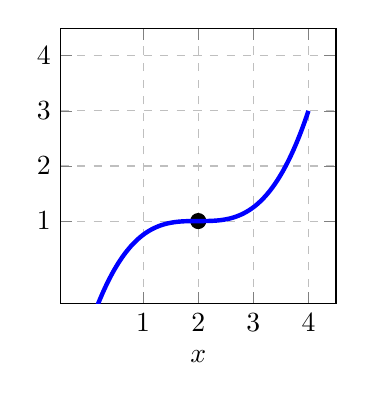
\begin{tikzpicture}[scale=1]
          \begin{axis}[
        %    axis y line = left,
        %    axis x line = bottom,
            xlabel={$x$},
            xtick       = {1,2,3,4},
            xticklabels = {1,2,3,4},
            ytick       = {1,2,3,4},
            yticklabels = {1,2,3,4},
            samples     = 160,
            domain      = -1:5,
            restrict y to domain=-1:5,
            xmin = -0.5, xmax = 4.5,
            ymin = -0.5, ymax = 4.5,
            grid=both, grid style=dashed,
            width=2in, height=2in
          ]
           \filldraw[black] (2,1) circle (2.5pt);
          \draw[thick] (2,1) circle (2.5pt);
          \addplot[domain=0:4, blue, ultra thick, mark=none] {.25*(x-2)^3+1};
        \end{axis}
    \end{tikzpicture}
    continuous at $2$
    \end{center}
\end{minipage}
%

%
\task \\ \begin{minipage}[t]{0.22\textwidth}
    \begin{center}
    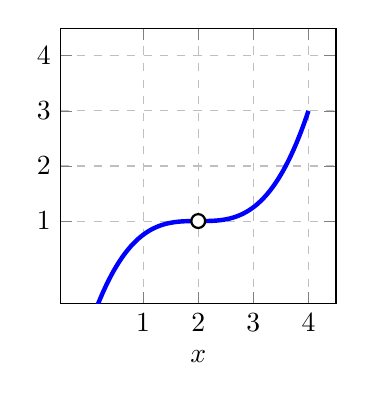
\begin{tikzpicture}[scale=1]
          \begin{axis}[
        %    axis y line = left,
        %    axis x line = bottom,
            xlabel={$x$},
            xtick       = {1,2,3,4},
            xticklabels = {1,2,3,4},
            ytick       = {1,2,3,4},
            yticklabels = {1,2,3,4},
            samples     = 160,
            domain      = -1:5,
            restrict y to domain=-1:5,
            xmin = -0.5, xmax = 4.5,
            ymin = -0.5, ymax = 4.5,
            grid=both, grid style=dashed,
            width=2in, height=2in
          ]
              
          \addplot[domain=0:4, blue, ultra thick, mark=none] {.25*(x-2)^3+1};
                \filldraw[white] (2,1) circle (2.5pt);
                \draw[thick] (2,1) circle (2.5pt);
                
        \end{axis}
    \end{tikzpicture}
    discontinuous at $2$ because only continuity conditions (1) \& (3) fail
    \end{center}
\end{minipage}
%

%
\task \\ \begin{minipage}[t]{0.22\textwidth}
    \begin{center}
    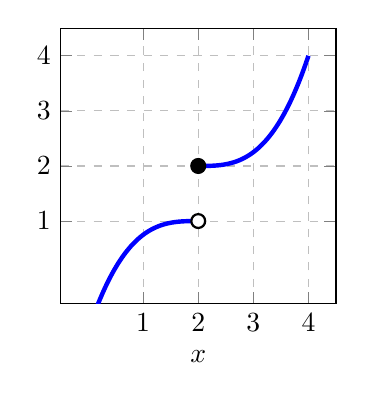
\begin{tikzpicture}[scale=1]
          \begin{axis}[
        %    axis y line = left,
        %    axis x line = bottom,
            xlabel={$x$},
            xtick       = {1,2,3,4},
            xticklabels = {1,2,3,4},
            ytick       = {1,2,3,4},
            yticklabels = {1,2,3,4},
            samples     = 160,
            domain      = -1:5,
            restrict y to domain=-1:5,
            xmin = -0.5, xmax = 4.5,
            ymin = -0.5, ymax = 4.5,
            grid=both, grid style=dashed,
            width=2in, height=2in
          ]
                    \addplot[domain=0:2, blue, ultra thick, mark=none] {.25*(x-2)^3+1};
                \filldraw[white] (2,1) circle (2.5pt);
                \draw[thick] (2,1) circle (2.5pt);
                 \addplot[domain=2:4, blue, ultra thick, mark=none] {.25*(x-2)^3+2};
                   \filldraw[black] (2,2) circle (2.5pt);
                \draw[thick] (2,2) circle (2.5pt);
        \end{axis}
    \end{tikzpicture}
    discontinuous at $2$ because only continuity conditions (2) \& (3) fail
    \end{center}
\end{minipage}
%

%
\task \\ \begin{minipage}[t]{0.22\textwidth}
\begin{center}
    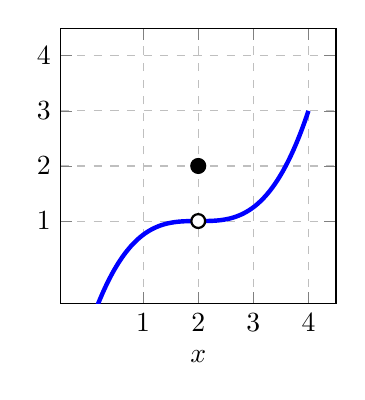
\begin{tikzpicture}[scale=1]
          \begin{axis}[
        %    axis y line = left,
        %    axis x line = bottom,
            xlabel={$x$},
            xtick       = {1,2,3,4},
            xticklabels = {1,2,3,4},
            ytick       = {1,2,3,4},
            yticklabels = {1,2,3,4},
            samples     = 160,
            domain      = -1:5,
            restrict y to domain=-1:5,
            xmin = -0.5, xmax = 4.5,
            ymin = -0.5, ymax = 4.5,
            grid=both, grid style=dashed,
            width=2in, height=2in
          ]
                              \addplot[domain=0:4, blue, ultra thick, mark=none] {.25*(x-2)^3+1};
                \filldraw[white] (2,1) circle (2.5pt);
                \draw[thick] (2,1) circle (2.5pt);
                   \filldraw[black] (2,2) circle (2.5pt);
                \draw[thick] (2,2) circle (2.5pt);
        \end{axis}
    \end{tikzpicture}
    discontinuous at $2$ because only continuity condition (3) fails
    \end{center}
\end{minipage}
}
%

\sol{
There are many, many reasonable answers. See above graphs for  a few options.
}

\end{document}